\documentclass{ximera}
%\documentclass[space,handout,nooutcomes]{ximera}

\newcommand{\N}{\mathbb N}
\newcommand{\W}{\mathbb W}
\newcommand{\C}{\mathbb C}
\newcommand{\Z}{\mathbb Z}
\newcommand{\Q}{\mathbb Q}
\newcommand{\R}{\mathbb R}

\title{Section 1.1 Problems}

\begin{document}
\begin{abstract}
Problems About Sets    
\end{abstract}
\maketitle


\begin{problem}
Given two sets $X$ and $Y$, explain what is meant by $X\cup Y$.
\begin{freeResponse}
$X\cup Y$ is the set of elements that are in $X$ or in $Y$ (or both, as the ``or'' is inclusive).  
\end{freeResponse}
\end{problem}

\begin{problem}
Given two sets $X$ and $Y$, explain what is meant by $X\cap Y$.
\begin{freeResponse}
$X\cap Y$ is the set of elements that are in $X$ and in $Y$.  
\end{freeResponse}
\end{problem}

\begin{problem}
Given two sets $X$ and $Y$, explain what is meant by $X - Y$.
\begin{freeResponse}
$X - Y$ is the set of elements that are in $X$ but not in $Y$.  
\end{freeResponse}
\end{problem}

\begin{problem}
Explain the difference between the symbols $\in$ and $\subset$.
\begin{freeResponse}
The notation $X \in Y$ would mean that $X$ is a single element in the set $Y$.  In this case, $X$ might not be a set.  Th notation $X \subset Y$ would require that both $X$ and $Y$ are sets and also that every element of $X$ is also in $Y$.
\end{freeResponse}
\end{problem}

\begin{problem}
How is $\{\emptyset\}$ different from $\emptyset$?  
\begin{freeResponse}
The empty set, $\emptyset$, is a set that contains no elements.  The set $\{\emptyset\}$ contains 1 element that is itself a set.  
\end{freeResponse}
\end{problem}

\begin{problem}
Draw a Venn diagram for the set of elements that are in $X$ or $Y$ \emph{but not both}. 
How does it differ from the Venn diagram for $X\cup Y$?  
\begin{freeResponse}
Same as the Venn diagram for $X\cup Y$, except that the $X\cap Y$ part is not shaded.  
\end{freeResponse}
\end{problem}

\begin{problem}
If we let $X$ be the set of ``right triangles'' and we let $Y$ be the set of ``equilateral triangles'' does the picture below show the relationship between these two sets?
\begin{image}
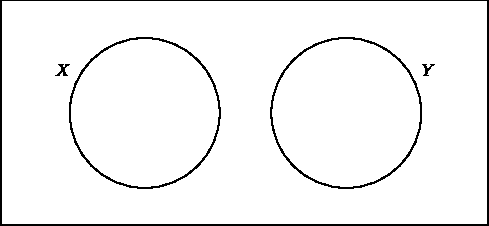
\includegraphics[scale=0.8]{set4.pdf}
\end{image}
Explain your reasoning.
\begin{freeResponse}
Yes.  The picture is accurate because no right triangles are also equilateral triangles.  
\end{freeResponse}
\end{problem}

\begin{problem}
If $X = \{1,2,3,4,5\}$ and $Y = \{3,4,5,6\}$ find:
\begin{enumerate}
\item $X\cup Y$
\item $X\cap Y$
\item $X-Y$
\item $Y-X$
\end{enumerate}
\begin{freeResponse}
\begin{enumerate}
\item[1] $X\cup Y = \{1,2,3,4,5,6\}$
\item $X\cap Y = \{3,4,5\}$
\item $X-Y = \{1,2\}$
\item $Y-X = \{6\}$
\end{enumerate}
\end{freeResponse}
\end{problem}

\begin{problem}
If $X\cup Y = X$, what can we say about the relationship between the sets $X$ and $Y$? Explain your reasoning.
\begin{freeResponse}
$Y\subset X$ because every element of $Y$ must already be in $X$.  
\end{freeResponse}
\end{problem}

\begin{problem}
If $X\cap Y = X$, what can we say about the relationship between the sets $X$ and $Y$? Explain your reasoning.
\begin{freeResponse}
$X\subset Y$ because every element of $X$ must already be in $Y$.  
\end{freeResponse}
\end{problem}

\begin{problem}
If $X-Y =\emptyset$, what can we say about the relationship between the sets $X$ and $Y$? Explain your reasoning.
\begin{freeResponse}
$X\subset Y$ because that would mean $X$ contains no elements that are not also in $Y$.  
\end{freeResponse}
\end{problem}



\end{document}
